\documentclass[report/main.tex]{subfiles}

A description and illustration of the:

% - Design of your ITU-MiniTwit systems
% - Architecture of your ITU-MiniTwit systems
% - All dependencies of your ITU-MiniTwit systems on all levels of abstraction and development stages.
    % - That is, list and briefly describe all technologies and tools you applied and depend on.
% - Important interactions of subsystems
% - Describe the current state of your systems, for example using results of static analysis and quality - assessment systems.
% - Finally, describe briefly, if the license that you have chosen for your project is actually compatible with - the licenses of all your direct dependencies.

% Double check that for all the weekly tasks (those listed in the schedule) you include the corresponding information.

\begin{document}
    \section{System's Perspective}
    \label{Sec:systems_perspective}
    
    \subsection{Design of the system}
    \label{subsec:design_of_system}
    % https://stackoverflow.com/questions/704855/software-design-vs-software-architecture

    \subsection{Architecture of the system}
    \label{subsec:architecture_of_system}
    % https://stackoverflow.com/questions/704855/software-design-vs-software-architecture
        TODO: the rest
        
        TODO: client server
        
        Following the principle of separation of concerns a Three Layered Architecture was chosen, thereby having separate programs for presentation tier (EvilClient), logic tier (EvilApi) and data tier (PSQL database). For reference see figure \ref{fig:three_layered:architecture}.
        

        \begin{wrapfigure}{r}{0.4\textwidth}
            \centering
            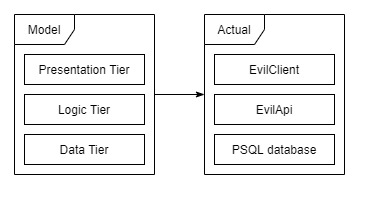
\includegraphics[width=0.4\textwidth]{report/images/MiniTwit-Three Layered Architecture.jpg}
            \caption{Caption}
            \label{fig:three_layered:architecture}
        \end{wrapfigure}

        As the application was split into two separate subsystem each subsystem will be covered separately starting with the EvilClient followed by the EvilApi
        
        \subsubsection{Architecture of EvilClient}
        \label{subsubsec:architexture_of_evilclient}
            The main responsibility of the EvilClient is to display data from the database to the user send by the EvilApi, and handle inputs to the user that could manipulate data in the database. Hence the responsibility of the EvilClient is data conversion between displaying data to the user, and converting user input to usable data in the database thereby, the MVVM (Model-View-ViewModel) pattern was chosen (\cite{ms-mvvm}).
            
            Of notice should be the Pages, Shared, ViewModels folders of the EvilClient folder. Here Pages and Shared contains the View part of MVVM which is handle by the Microsoft Blazor Framework\footnote{\hyperlink{https://dotnet.microsoft.com/apps/aspnet/web-apps/blazor}{https://dotnet.microsoft.com/apps/aspnet/web-apps/blazor}} to convert the code into a application that is executable in a web browser. The ViewModels folder holds the code that converts data from the EvilApi into usuable information to the user, and vice verse converts input from the client into data that is usable for the EvilApi.

        \subsubsection{Architecture of EvilApi}
        \label{subsubsec:architecture-of-evilApi}
            EvilApi is a simple REST Api (\cite{rest}) that handles request via the Microsoft ControllerBase (\cite{ms-web-api}), and updates a PostgreSQL database via EF Core\footnote{\hyperlink{https://docs.microsoft.com/en-us/ef/core/}{https://docs.microsoft.com/en-us/ef/core/}}. Hence it would receive http request, send them to
    
    \subsection{Dependencies}
    \label{subsec:dependencies}
        \begin{table}[h!]
    \small
    \caption {Dependencies grouped by license} \label{tab:title}
    \begin{tabular}{|l|l|l|l|}
    \hline
    apache 2                            & MIT                           & BSD 3clause & PostgresQL license \\ \hline
    AspNetCore.Diagnostics.HealthChecks & Newtonsoft.Json               & moq4        & npgsql/efcore.pg   \\
    code-cracker                        & ProfanityDetector             &             &                    \\
    dotnet/efcore                       & prometheus-net                &             &                    \\
    aspnet/Diagnostics                  & prometheus-net.SystemMetrics  &             &                    \\
    serilog-aspnetcore                  & RehanSaeed/Serilog.Exceptions &             &                    \\
    serilog-enrichers-environment       & Swashbuckle.AspNetCore        &             &                    \\
    serilog-sinks-debug                 & coverlet                      &             &                    \\
    serilog-sinks-elasticsearch         & vstest                        &             &                    \\
    Roslynator                          &                               &             &                    \\
    xunit                               &                               &             &                    \\
    visualstudio.xunit                  &                               &             &                    \\ \hline
    \end{tabular}
    \end{table}

    
    
    \subsection{Interactions of subsystems}
    
    \subsection{Current state of the systems}
    
    \begin{itemize}
        \item \textbf{} \url{https://sonarcloud.io/dashboard?id=gustavjohansen98_E-vil-Corp}
    \end{itemize}
    
    \subsection{Software license agreement}
    As listed in section \ref{subsec:dependencies}, we have 21 direct dependencies. 11 of them are licensed under Apache version 2\footnote{https://www.apache.org/licenses/LICENSE-2.0}, 8 of them under the MIT license\footnote{https://opensource.org/licenses/MIT}, while the BSD 3-clause\footnote{https://opensource.org/licenses/BSD-3-Clause} and PostgresQL license\footnote{https://www.postgresql.org/about/licence/} cover 1-1 dependency each. Since all of these licences are permissive, we had a lot of freedom to choose how to license our software. While we must preserve the original license notices in the files which use code covered by the aforementioned licences, we are permitted to license the project \textit{as a whole} as we see fit. Therefore, to make sure evil capitalists don't profit from our work, we released the project under the GPL version 3\footnote{https://www.gnu.org/licenses/gpl-3.0.en.html}.
    


\end{document}